\documentclass[tikz,border=12pt]{standalone}
\usepackage{amsmath,amssymb}
\usetikzlibrary{calc,arrows.meta}

\begin{document}
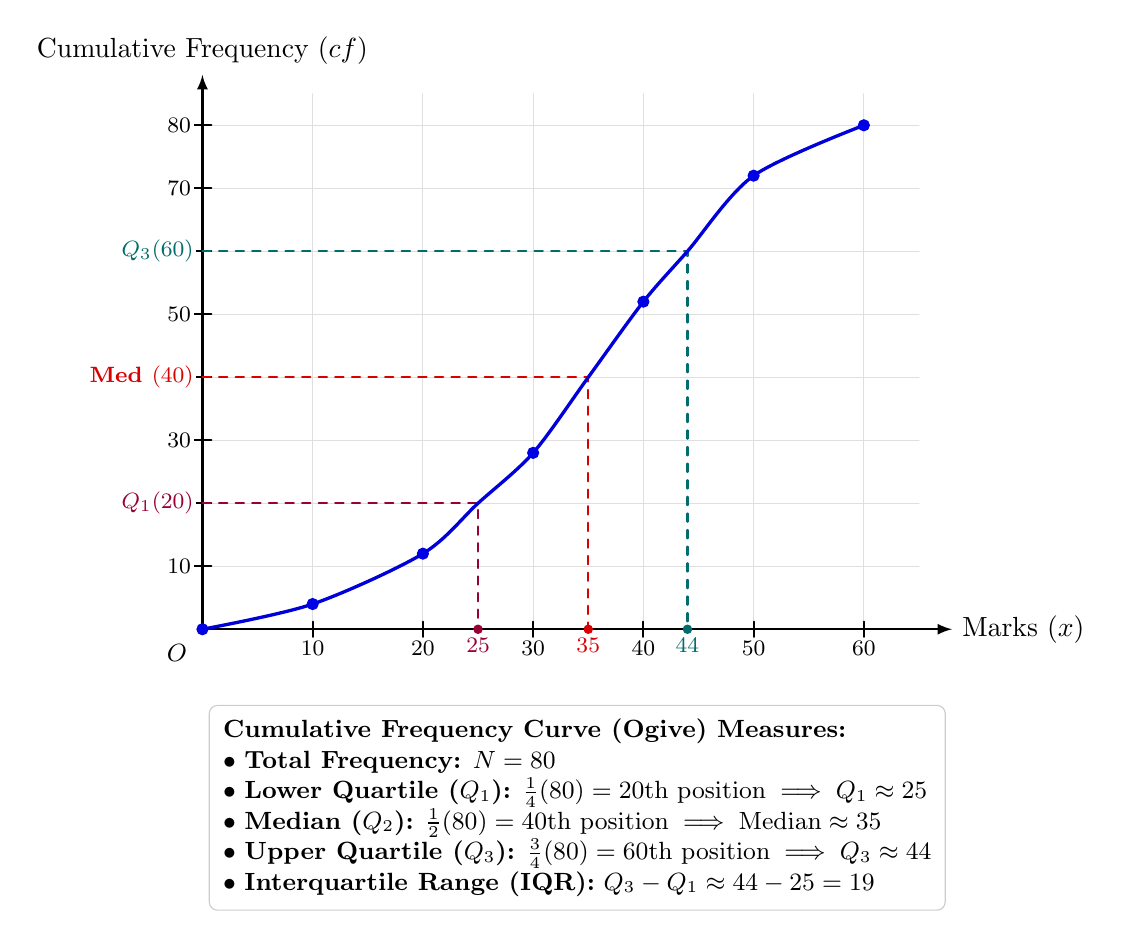
\begin{tikzpicture}[>=latex, line cap=round, line join=round, x=0.14cm, y=0.08cm]

  % Millimeter / Grid background
  \draw[step=10, gray!25, thin] (0, 0) grid (65, 85);

  % Axes
  \draw[thick, ->] (0, 0) -- (68, 0) node[right, font=\normalsize] {Marks ($x$)};
  \draw[thick, ->] (0, 0) -- (0, 88) node[above, font=\normalsize] {Cumulative Frequency ($cf$)};

  % Origin
  \node[below left=2pt, font=\small] at (0, 0) {$O$};

  % Integer ticks on x-axis
  \foreach \x in {10, 20, 30, 40, 50, 60} {
    \draw[thick] (\x, 1.2) -- (\x, -1.2);
    \node[below=3pt, font=\footnotesize, fill=white, inner sep=1pt] at (\x, 0) {$\x$};
  }

  % Integer ticks on y-axis
  \foreach \y in {10, 20, 30, 40, 50, 60, 70, 80} {
    \draw[thick] (0.8, \y) -- (-0.8, \y);
    \node[left=3pt, font=\footnotesize, fill=white, inner sep=1pt] at (0, \y) {$\y$};
  }

  % Quartile projections (dashed lines)
  % Lower Quartile Q1 (cf = 20 -> x = 25)
  \draw[thick, dashed, purple!80!black] (0, 20) -- (25, 20) -- (25, 0);
  \node[left=2pt, font=\footnotesize\bfseries, purple!80!black, fill=white, inner sep=1pt] at (0, 20) {$Q_1 (20)$};
  \filldraw[purple!80!black] (25, 0) circle (1.5pt) node[below=2pt, font=\footnotesize\bfseries, fill=white, inner sep=1pt] {$25$};

  % Median Q2 (cf = 40 -> x = 35)
  \draw[thick, dashed, red!85!black] (0, 40) -- (35, 40) -- (35, 0);
  \node[left=2pt, font=\footnotesize\bfseries, red!85!black, fill=white, inner sep=1pt] at (0, 40) {Med $(40)$};
  \filldraw[red!85!black] (35, 0) circle (1.5pt) node[below=2pt, font=\footnotesize\bfseries, fill=white, inner sep=1pt] {$35$};

  % Upper Quartile Q3 (cf = 60 -> x = 44)
  \draw[thick, dashed, teal!85!black] (0, 60) -- (44, 60) -- (44, 0);
  \node[left=2pt, font=\footnotesize\bfseries, teal!85!black, fill=white, inner sep=1pt] at (0, 60) {$Q_3 (60)$};
  \filldraw[teal!85!black] (44, 0) circle (1.5pt) node[below=2pt, font=\footnotesize\bfseries, fill=white, inner sep=1pt] {$44$};

  % Smooth Ogive Curve
  \draw[very thick, blue!85!black, smooth] plot coordinates {
    (0, 0) (10, 4) (20, 12) (25, 20) (30, 28) (35, 40) (40, 52) (44, 60) (50, 72) (60, 80)
  };

  % Data plot points
  \foreach \p in {(0,0), (10,4), (20,12), (30,28), (40,52), (50,72), (60,80)} {
    \filldraw[blue!90!black] \p circle (2pt);
  }

  % Summary Card
  \node[align=left, font=\small, fill=white, inner sep=5pt, draw=gray!40, rounded corners=3pt, anchor=north] at (34, -12) {
    \textbf{Cumulative Frequency Curve (Ogive) Measures:}\\
    $\bullet$ \textbf{Total Frequency:} $N = 80$\\
    $\bullet$ \textbf{Lower Quartile ($Q_1$):} $\frac{1}{4}(80) = 20\text{th position} \implies Q_1 \approx 25$\\
    $\bullet$ \textbf{Median ($Q_2$):} $\frac{1}{2}(80) = 40\text{th position} \implies \text{Median} \approx 35$\\
    $\bullet$ \textbf{Upper Quartile ($Q_3$):} $\frac{3}{4}(80) = 60\text{th position} \implies Q_3 \approx 44$\\
    $\bullet$ \textbf{Interquartile Range (IQR):} $Q_3 - Q_1 \approx 44 - 25 = 19$
  };

\end{tikzpicture}
\end{document}
